\documentclass[12pt]{article}

\usepackage{graphicx}
\usepackage{epstopdf}


\usepackage[spanish]{babel} % silabea palabras castellanas <- Puedo poner comentarios para explicar de que va este comando en la misma línea
\selectlanguage{spanish} 

%Encoding
\usepackage[utf8]{inputenc} % Acepta caracteres en castellano
\usepackage[T1]{fontenc} % Encoding de salida al pdf

%Triunfó el mal
\usepackage[normalem]{ulem}
\useunder{\uline}{\ul}{}
\providecommand{\e}[1]{\ensuremath{\times 10^{#1}}}
\usepackage{quotmark} %Uso consistente con la RAE de comillas
\usepackage{listings} % Comandos de la terminal

\usepackage{textcomp}
\usepackage{gensymb}


%Hipertexto
\usepackage[colorlinks=true,urlcolor=blue,linkcolor=blue]{hyperref} % navega por el doc: hipertexto y links

%Aquello de las urls
\usepackage{url} 

%simbolos matemáticos
\usepackage{amsmath}
\usepackage{amsfonts}
\usepackage{amssymb}
\usepackage{physics} %Best pack

% permite insertar gráficos, imágenes y figuras, en pdf o en eps
\usepackage{graphicx}
\usepackage{epstopdf}
\usepackage{multirow}
\usepackage{float}
\usepackage[export]{adjustbox}
% geometría del documento, encabezados y pies de páginas, márgenes
\usepackage{geometry}
\usepackage{comment}

%\usepackage[english]{babel}
%\usepackage[latin5]{inputenc}
% \usepackage{hyperref}
%\newdate{date}{10}{05}{2013}
%\date{\displaydate{date}}
\begin{document}




\title{Cúmulos Abiertos \\ Taller 3 Fotometría de Apertura IRAF}

\author{
\textbf{Javier Alejandro Acevedo Barroso\thanks{e-mail: \texttt{ja.acevedo12@uniandes.edu.co}}}\\
\textit{Universidad de los Andes, Bogotá, Colombia}\\
 }% Hasta aquí llega el bloque "author" (son dos autores por informe, orden alfabético)

\date{\today}
%\date{Versión $\alpha \beta$ fecha del documento}
\maketitle %Genera el título del documento


\normalsize
\newpage


\section{Función Inicial de Masa}
La función inicial de masa es la función que relaciona la masa al momento de entrar a la secuencia principal, con el número de estrellas en una población entrando a la secuencia principal con esa masa. Es decir, en una población estelar recien nacida de estrellas, la función inicial de masa correspondería completamente con el histograma de las masas. La importancia de la función inicial de masa radica en que la masa con la que una estrella entra a su secuencia principal es la variable más importante para determinar su evolución.\\



\section{Fotometría de apertura}
El objetivo de este ejercicio es realizar el procesamiento de fotometría de apertura para las imágenes del tutorial de IRAF. Esto corresponde a calcular una magnitud instrumental para los objetos del campo estelar. Por ser la primera vez que se realiza tal análisis, se realizará paso a paso y para un número límitado de estrellas. En futuros ejercicios se realizará el análisis para todo el campo, usando algoritmos implementados en IRAF para localizar los objetos.\\

Las imágenes se tomaron con instrumentos CCD y por lo tanto se realizaron las respectivas correcciones de FLAT, OVERSCAN y BIAS. El ejercicio asume que las imágenes ya están corregidas.\\


El primer paso va a ser añadir al header de las imágenes la masa de aire. El cálculo de la masa de aire requiere de cierta información, como la posición del observatorio o la coordenada exacta en el cielo del objeto. Afortunadamente IRAF incluye una tarea titulada SETAIRMASS la cual lee toda la información necesaria del header de la imagen. Usando la tarea SETAIRMASS y señalando que estamos en el observatorio kpno (Kitt Peak National Observatory), se fija en el header de cada imagen la masa de aire. Se observa que la masa de aire para las imágenes de calibración es de aproximadamente 2, esa masa de aire es irrelevante pues las imágenes de calibración no son tomas del cielo. Las masas de aire para las imágenes reales en el filtro V es 1.07 y en el filtro B 1.09.\\

Una vez fijada las masas de aire, se procede a hacer la fotometría de apertura. Para ello se utiliza el paquete DIGIPOT y APPHOT. La fotometría se realizará sobre los objetos que creemos ser estrellas. Es decir, se evaluarán las curvas de intensidad radiales en cada objeto, y solo se tomará los de mejor perfil. Esto se hace con la tarea IMEXAMINE. Se observa que las estrellas tienen un FWHM de 2.65 a 3.2 y que es constante entre las diferentes imágenes.\\

Para realizar la fotometría en sí se usa la tarea QPHOT. Esta necesita el radio de apertura, el radio interior del anillo de cielo y el grosor del anillo de cielo, todo esto en pixeles. Tras ejecutar la tarea QPHOT sobre la imagen m92010, se obtiene una tabla de objetos con sus coordenadas, su magnitud, y error (si hubo). Usando la tarea txdump se extrae las coordenadas de las estrellas seleccionadas (se seleccionó a las estrellas en el modo interactivo de QPHOT). Una vez se tiene las coordenadas de las estrellas, se vuelve a correr QPHOT sobre las otras imágenes. Se seleccionaron 30 estrellas (ver figura \ref{im4}) para realizar la fotometría.



\begin{figure}[H]
   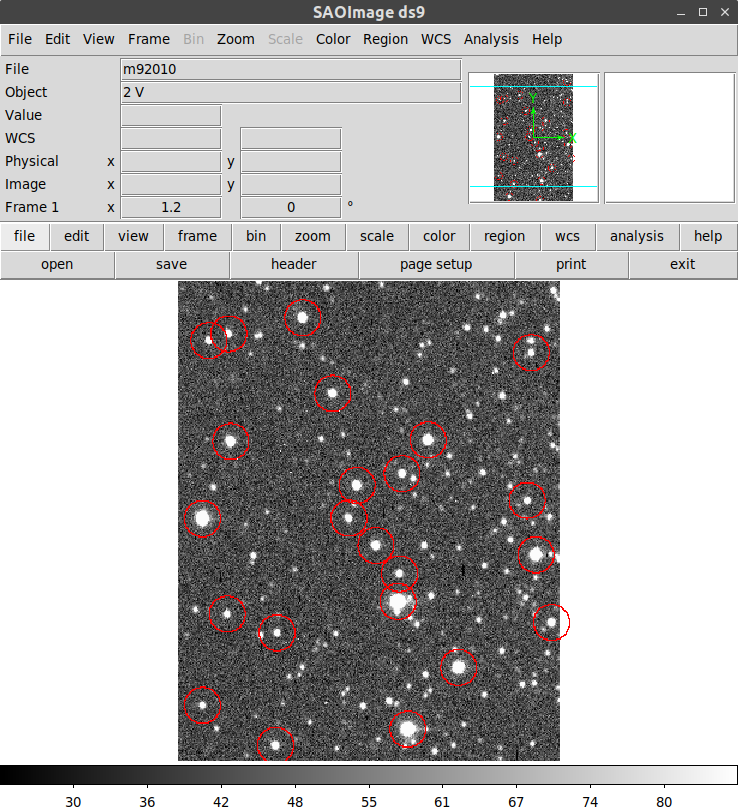
\includegraphics[scale=0.4]{imagenes.png}
  \caption{Estrellas seleccionadas para la fotometría de apertura en la imagen m92010.}
  \label{im4}
\end{figure}

Adicionalmente, para cada imagen se graficó la magnitud contra el error de la magnitud, de un análisis correcto se espera un comportamiento cuadrático en la gráfica $m$ vs $\Delta m $. Se observó el comportamiento cuadrático en todas las gráficas (ver figura \ref{im5}).\\


Por último, para verificar que el comportamiento cuadrático se debe a un análisis correcto, se calculó la magnitud y el error en la magnitud para coordenadas aleatorias del cielo, procurando no tomar estrellas. Se observó un comportamiento muy levemente cuadrático (probablemetne un remanente de las estrellas que sí quedaron a dentro de los circulos) y una gran cantidad de puntos indeterminados, debido a que el algoritmo no logra hayar una magnitud en esas coordenadas.

\begin{figure}[H]
   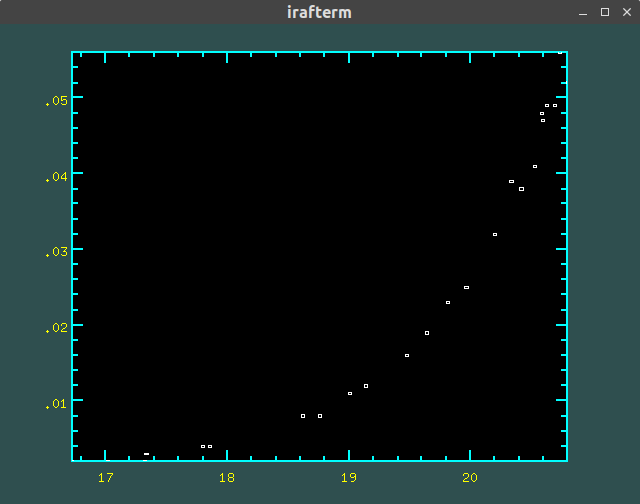
\includegraphics[scale=0.4]{mvsdm0.png}
   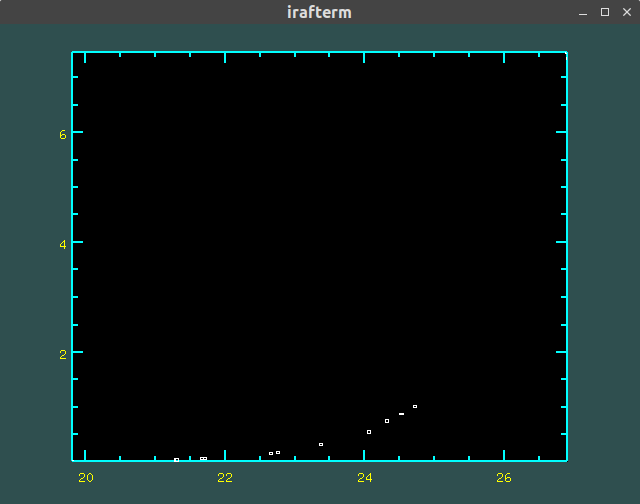
\includegraphics[scale=0.4]{mvsdm1.png}

  \caption{ A la izquierda magnitud contra error en la magnitud para las estrellas en la imagen m92010. Se observa un comportamiento cuadrático. Se anexa únicamente el caso de m92010 porque las otras gráficas son muy similares. A la derecha la misma gráfica pero para puntos que no correspondieran a estrellas, la disminución de puntos se debe a que el algoritmo no converge en muchas ocasiones debido al ruido de fondo.}
  \label{im5}
\end{figure}



\newpage
\section{BIAS}
Como parte del proyecto del curso se debe realizar algunas tomas con el telescopio y el instrumento CCD disponible. Por ello, es necesario hacer calibración de FLAT y de BIAS. Se decidió empezar con la calibración de BIAS.\\

La calibración de BIAS consiste en tomar los valores del detectos sin tiempo de exposición, esto para para dar cuenta del ruido intrínseco del detectos (nótese que el ruido puede variar entre pixeles).\\

Se tomó 30 imágenes de calibración BIAS a diferentes temperaturas: 0 \degree C, -5 \degree C, -10 \degree C y -14 \degree C. Se calculó la mediana de las 30 imágenes para cada temperatura y se generó una nueva imágen con las medianas, esa nueva imagen es la corrección de BIAS a la temperatura correspondiente.\\

Una vez generada la imagen de medianas para cada temperatura, se comparó el promedio de sus filas. Esto con el fin de buscar anomalías (picos) en el detector.\\





\bibliography{bibTes}{}
\bibliographystyle{unsrt}


\begin{figure}[H]
   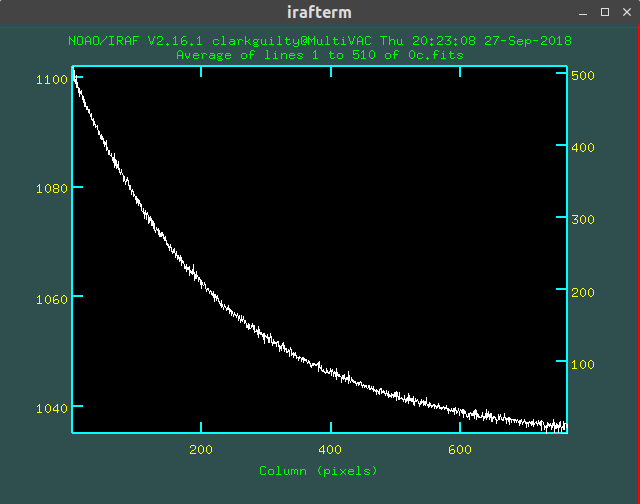
\includegraphics[scale=0.4]{0c.png}
   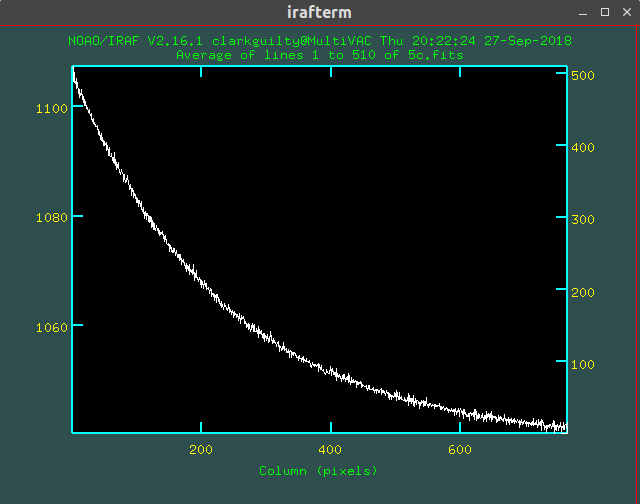
\includegraphics[scale=0.4]{5c.png}
  \caption{Promedio de conteos sobre todas las líneas para 0 \degree C y -5 \degree C }
  \label{im0}
\end{figure}



\begin{figure}[H]
   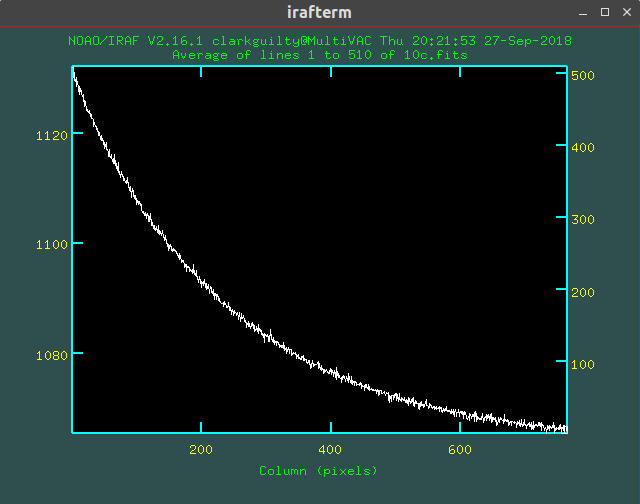
\includegraphics[scale=0.4]{10c.png}
   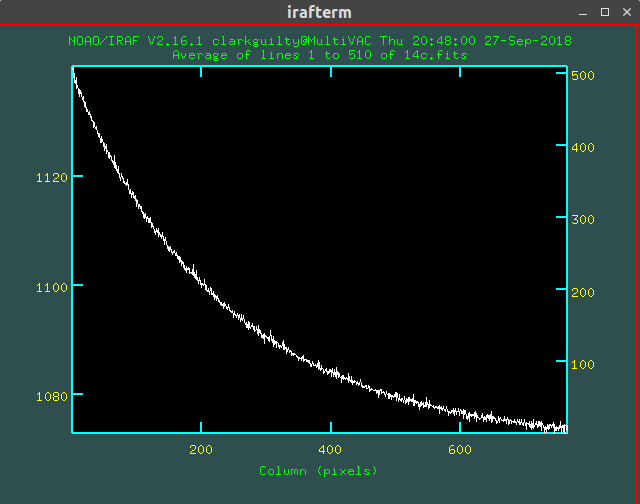
\includegraphics[scale=0.4]{14c.png}
  \caption{Promedio de conteos sobre todas las líneas para -10 \degree C y -14 \degree C. }
  \label{im1}
\end{figure}
No se observa ningún pico particular en los promedios. Sin embargo, se observa que tienen diferentes límites las curvas, implicando diferentes medianas. Adicionalmente  se observa una forma general similar entre las curvas.\\

También se comparó la media de conteos contra la temperatura (ver figura \ref{imMedias}) , se observa un aumento de conteos al \emph{disminuir} la temperatura. El comportamiento del número de conteos implica una temperatura de operación óptima de 0 \degree C o superior.



\begin{figure}[H]
   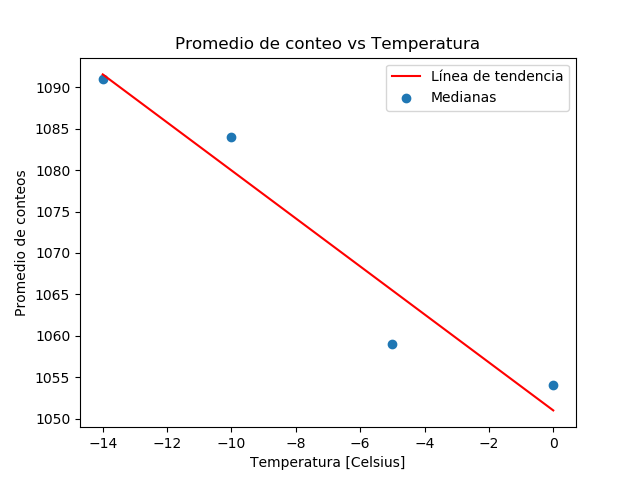
\includegraphics[scale=0.7]{medias.png}
  \caption{Promedio de conteos contra temperatura. La línea de tendencia es de una de mínimos cuadrados y está únicamente como ayuda de visualización. }
  \label{imMedias}
\end{figure}










\end{document}




\begin{figure}[H]
  \centering
   \includegraphics[scale=•]{•}= 0.65]{im03.png}
  \caption{Cargando las imágenes a diferentes frames de DS9 desde la sesión de IRAF. }
  \label{im03}
\end{figure}





\section{Cronograma}

\begin{table}[htb]
	\begin{tabular}{|c|cccccccccccccccc| }
	\hline
	Tareas $\backslash$ Semanas & 1 & 2 & 3 & 4 & 5 & 6 & 7 & 8 & 9 & 10 & 11 & 12 & 13 & 14 & 15 & 16  \\
	\hline
	1 & X & X & X  &   &   &   &   &  &  &   &   &   &   &   &   &   \\
	2 &   &  & X & X & X &  &  &   &   &  &  &  &   &  &  &   \\
	3 &   &   &   &  & X  & X  & X  & X &   &   &   &  &   &   &  &   \\
	4 &  &  &  &  &  &  &  & X & X & X & X &   &   &   &   &   \\
    5 &  &  &  &  &  &  & X & X &  &  &  &   &   &   &   &   \\
	6 &   &   &   &   &  &   &  X & X  &  &   &  X & X &  X & X  & X &   \\
	\hline
	\end{tabular}
\end{table}
\vspace{1mm}
 %CCDRED se encarga de la corrección en sí, sus parámetros son: el tipo de dato de los pixeles (real, short, etc), el nombre del backup (en caso de querer un backup), el archivo de traducción del instrumento (que para una CCD estandar ya viene incluido en IRAF